\documentclass[20pt,margin=1in,innermargin=-4.5in,blockverticalspace=-0.25in]{tikzposter}
\geometry{paperwidth=42in,paperheight=30in}
\usepackage[utf8]{inputenc}
\usepackage{amsmath}
\usepackage{amsfonts}
\usepackage{amsthm}
\usepackage{amssymb}
\usepackage{caption}
\usepackage{mathrsfs}
\usepackage{graphicx}
\usepackage{adjustbox}
\usepackage{enumitem}
\usepackage[backend=biber,style=numeric]{biblatex}
\usepackage{emory-theme}
\usepackage[scaled]{helvet}
\usepackage[T1]{fontenc}
\usepackage{tikz}
\usepackage{wrapfig}
\usetikzlibrary{shapes.geometric,calc}


\usepackage{mwe} % for placeholder images

\addbibresource{refs.bib}

% Set theme parameters,
\tikzposterlatexaffectionproofoff
\usetheme{EmoryTheme}
\usecolorstyle{EmoryStyle}

% Implement table environment, since this is not part of the 'tikzposter' package.
% For reference see: 
% https://tex.stackexchange.com/questions/337953/tikzposter-table-environment
\makeatletter
\newcounter{tablecounter}
\newenvironment{tikztable}[1][]{
	\def \rememberparameter{#1}
	\vspace{10pt}
	\refstepcounter{tablecounter}
	\begin{center}
	}{
		\ifx\rememberparameter\@empty
		\else
		\\[10pt]
		{\small Tab.~\thetablecounter: \rememberparameter}
		\fi
	\end{center}
}
\makeatother

% Additional commands.
% Score counter.
\newcommand\score[2]{%
	\pgfmathsetmacro\pgfxa{#1 + 1}%
	\tikzstyle{scorestars}=[star, star points=5, star point ratio=5, draw, inner sep=1.3pt, anchor=outer point 3]%
	\begin{tikzpicture}[baseline]
		\foreach \i in {1, ..., #2} {
			\pgfmathparse{\i<=#1 ? "yellow" : "gray"}
			\edef\starcolor{\pgfmathresult}
			\draw (\i*1.75ex, 0) node[name=star\i, scorestars, fill=\starcolor]  {};
		}
	\end{tikzpicture}%
}


% Header
\title{Parallelization in Multiple Imputation}
\author{Sven Nekula, Joshua Simon and Eva Wolf}
\institute{Otto Friedrich University, Bamberg}
\titlegraphic{
\includegraphics[width=0.06\textwidth]{img/uni_ba_logo_100_blau.png}}

% Begin document.
\renewcommand\familydefault{\sfdefault}
\begin{document}
\maketitle
\centering

\begin{columns}
    \column{0.32}
    \block{What is Parallelization?}{
    	\begin{wrapfigure}{l}{5cm}
    		\centering
    	    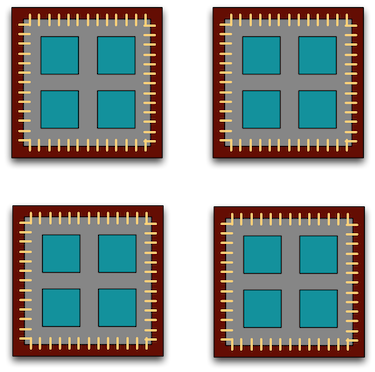
\includegraphics[width=5cm]{img/cpu.png}
    	    \caption{4 processors with 4 cores each \cite{cite:mattjones}}
    	\end{wrapfigure}
		
        \textcolor{earthyellow}{\textbf{Parallelization}} is a technique to fasten time-consuming computations. It uses several  cores on a \textbf{CPU} parallely and splits up the computational work between the cores. Afterwards, the results are merged. This can reduce the runtime significantly. The use of parallelization is however limited to certain tasks: The computations to be parallelized must be independent from each other, as information cannot be cross-accessed over the cores while the process is running.\\
    }

	\block{Theory}{
		\begin{wrapfigure}{r}{15cm}
			\centering
			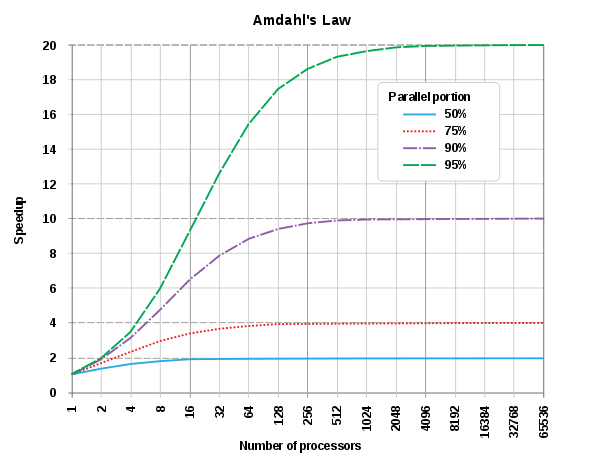
\includegraphics[width=15cm]{img/600px-AmdahlsLaw.svg}
			\caption{Amdahl's Law \cite{cite:mattjones}}
		\end{wrapfigure}

		In \textcolor{earthyellow}{\textbf{parallel programming}}, the multiple cores of a computational system want to be used best to decrease computation time. Gene \textbf{Amdahl} was the first one to desribe the boundaries of that project: Every parallel process also requires additional workload, so called "data management housekeeping". The speed up through parallel processing will tend to $0$ at a certain amount of processing units involved, as this \textbf{overhead} workload exceeds the capacity of the computational unit which it is assigned to \cite{cite:mattjones}.\\
		\textcolor{earthyellow}{\textbf{Multiple imputation MI}} is a method to complete a dataset with missing data. It relies on the estimation of the missing values through different methods. What is common to them is that not a single imputation run is used, but several. The results of all imputation runs are then merged and lead to realistic uncertainty of the estimators given the missing data. It is prone to be parallelized, as the several imputation runs can be processed independend of each other on different cores and easily merged afterwards \cite{van2018flexible}.
	}

	\block{Methodology}{
		As the \textcolor{earthyellow}{\textbf{dataset}} we used a simple data generator of normally distributed random variables. The data set created contains $10$ variables, some of which depend on each other. The sample size is $n = 10000$. Parallelization favors complex data sets, so the amount of variables and their interdependency should not be to small.\\
		\textcolor{earthyellow}{\textbf{Time measurement}} was done with the \textit{system.time} function, which returns three values: User CPU-, User System- and Elapsed time. User CPU is the time needed for the current task such as an execution in R. System CPU describes the time needed by the operating system to organize that task such as opening folders or asking for the System time. Elapsed time is the wall clock time that passed while the function and background processes were running.\\
		The \textcolor{earthyellow}{\textbf{method}} of the \textcolor{earthyellow}{\textbf{mice}} algorithm was set on defaut for numeric data, pmm \cite{van2018flexible}.\\
		The \textcolor{earthyellow}{\textbf{speed up}} value is calculated by the serial time (runtime without parallelization) divided by the runtime of the current parallelization implementation \cite{cite:chapple2016mastering}. Values below one show that the parallelized run took longer than the serial run.\\
	}

	
    \column{0.36}
    \block{Results}{
		\vspace{1em}
		\begin{tikzfigure}
			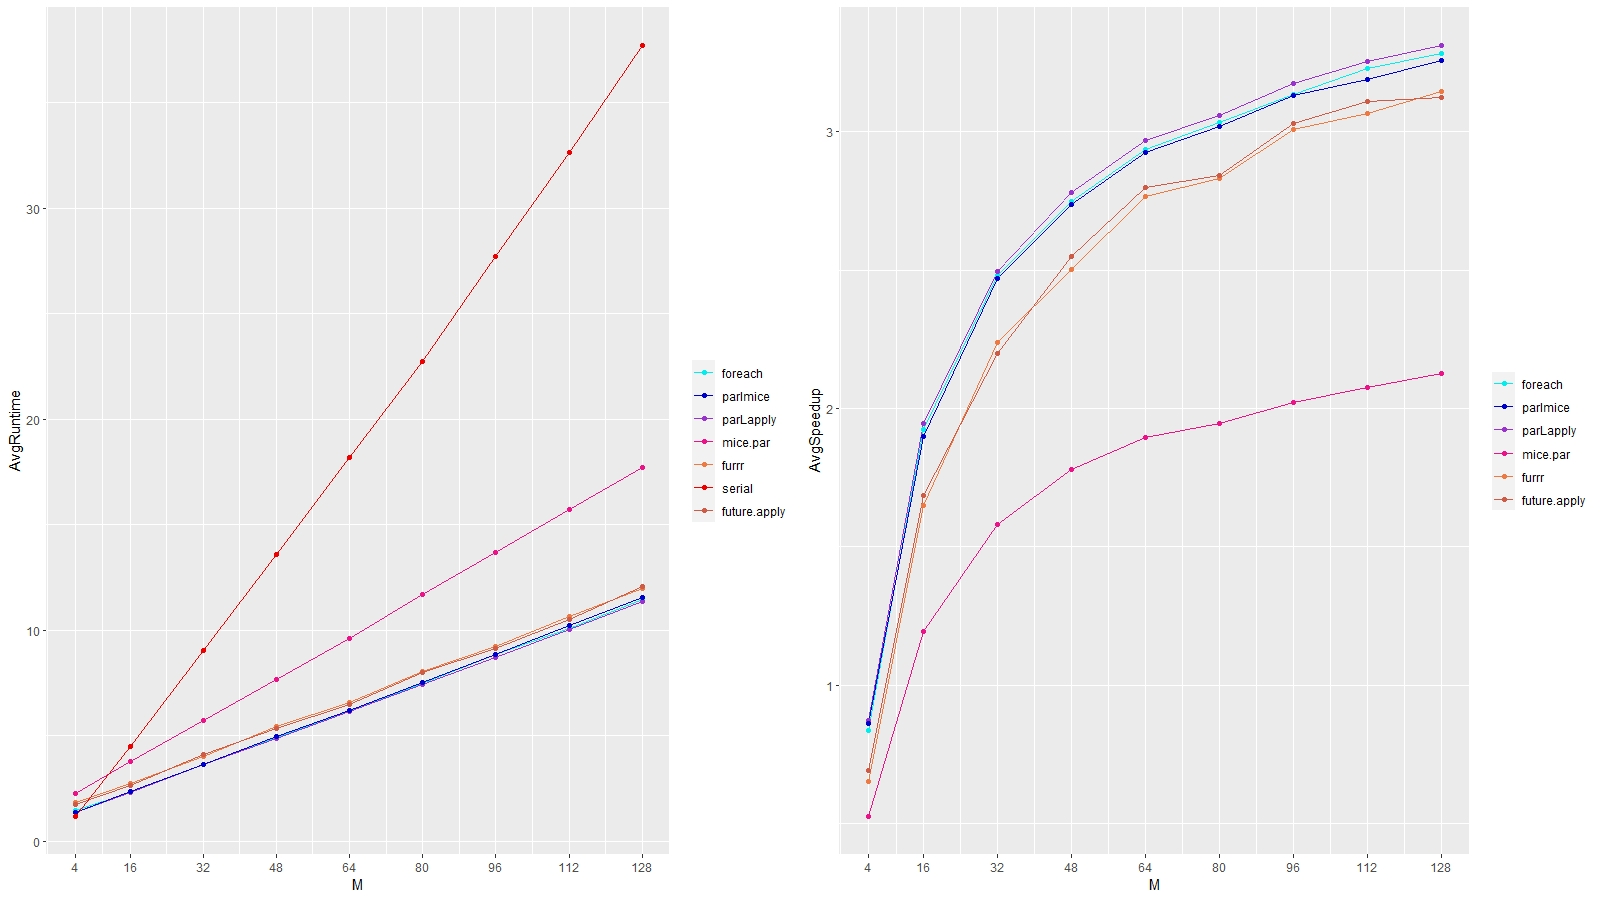
\includegraphics[width=1\linewidth]{img/different_m_comparison}
			\captionof{figure}{Runtime and Speedup from $4$ up to $128$ Imputation runs on a quad-core CPU}
		\end{tikzfigure}
       	\vspace{1em}
		
        \vspace{1em}
		\begin{tikzfigure}
			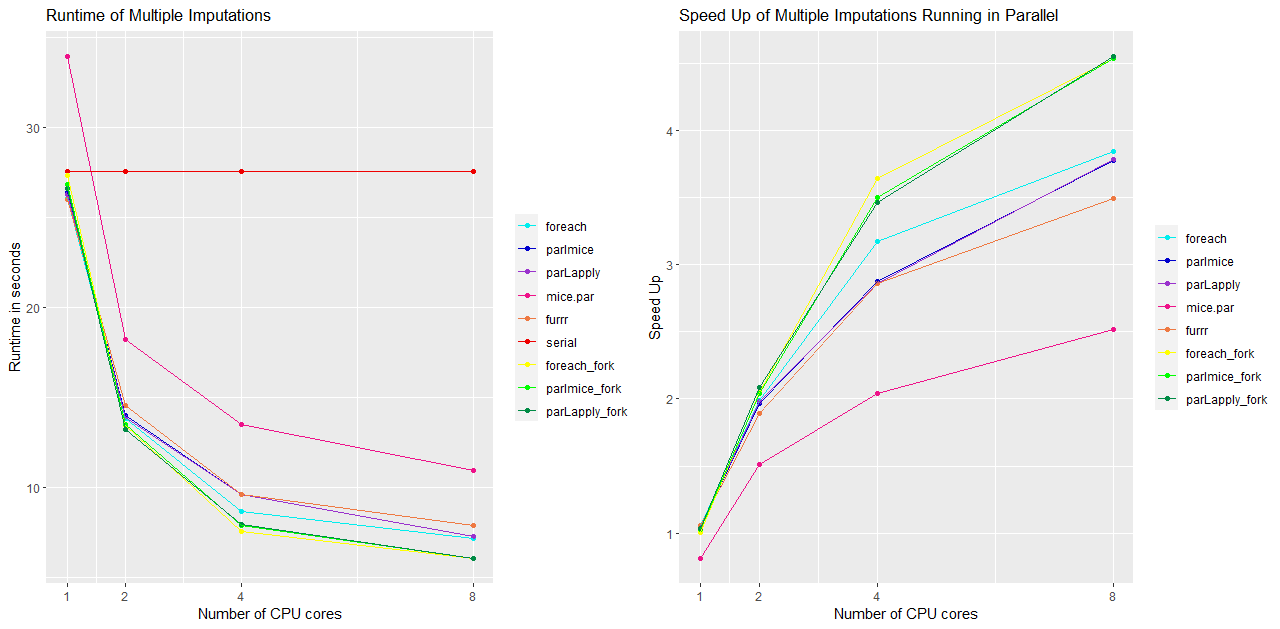
\includegraphics[width=1\linewidth]{img/runtime_ncores_speedup}
			\captionof{figure}{Runtime and Speedup from $1$ up to $16$ cores for $M = 128$ imputations}
		\end{tikzfigure}
        \vspace{1em}
       
      	\vspace{1em}
		\begin{tikztable}%[Time components for the different implementations for $M = 128$ imputations]
			%\small		% reduce font size within the table
			\begin{tabular}{rlrrrrrr}
				\hline
				& Function & Cores \vline & & & Average & & \\ 
				\hline
				& & \vline & User Time & System Time & Elapsed Time & Speed Up & Parallelism\\
				\hline
				\hline
				1 & foreach & $16$ & $0.25$ & $0.03$ & $7.63$ & $4.48$ & $0.83$ \\ 
				2 & foreach\_fork & $16$ & $0.21$ & $0.17$ & $7.03$ & $5.15$ & $0.85$ \\ 
				3 & furrr & $16$ & $1.07$ & $0.09$ & $8.93$ & $3.83$ & $0.79$ \\ 
				4 & future.apply & $16$ & $0.89$ & $0.07$ & $7.99$ & $3.90$ & $0.79$ \\ 
				5 & mice (serial) & $16$ & $31.04$ & $0.06$ & $31.11$ & $1.00$ &  - \\ 
				6 & mice.par & $16$ & $1.15$ & $0.10$ & $13.67$ & $2.50$ & $0.64$ \\ 
				7 & parLapply & $16$ & $0.33$ & $0.04$ & $7.80$ & $4.39$ & $0.82$ \\ 
				8 & parLapply\_fork & $16$ & $0.23$ & $0.17$ & $6.40$ & $5.36$ & $0.87$ \\ 
				9 & parlmice & $16$ & $0.30$ & $0.02$ & $7.76$ & $4.41$ & $0.82$ \\ 
				10 & parlmice\_fork & $16$ & $0.21$ & $0.18$ & $6.54$ & $5.25$ & $0.86$ \\ 
					\hline
				\end{tabular}
				\captionof{table}{Time components for the different implementations for $M = 128$ imputations}
		\end{tikztable}
    	\vspace{1em} 
    }


    \column{0.32}
    \block{Further Applications}{
    %\begin{wrapfigure}{r}{6cm}
    %	
\includegraphics[width=5cm]{img/disk.framing}
    %\end{wrapfigure}
	The opposite case to paralellized processes is the intended time-intensive, serial processing of Big Data with \textcolor{earthyellow}{\textbf{disk framing}}. In that setting we have data that exceeds the \textbf{RAM capacity} of the system, so that the data needs to a split up into several smaller chunks. These are then processed in portions that fit the available memory. Nevertheless, also for \textbf{disk framing}, parallelization is a useful tool to decrease computation time. The system chooses as many chunks of data as they fit into the RAM and then processes them in parallel, so that use of the computational power of the system can be made, while the memory capacity limits the speed by the amount of data which is processed at once. \cite{cite:diskframe} \\

	Considering today's trends in parallel and high performance computing, \textcolor{earthyellow}{\textbf{scalability}} plays a big role. So-called distributed systems are used here. These can be seen as the fusion of several computers into one system, often referred to as a \textbf{computing cluster}. In order to run a computer program on such an architecture, a \textbf{message passing interface (MPI)} is used, which now handles the communication between multiple CPUs and their cores. Popular applications are cloud solutions like Amazon's AWS (Amazon Web Services). The R language can make use of MPI with packages like \textbf{Rmpi} or \textbf{pbdMPI} \cite{cite:chapple2016mastering} and together with the \textbf{OpenMPI} implementation utilize the lower level of parallelism. \cite{cite:robey2021parallel}
	
	}

	\block{Conclusion}{
		\begin{itemize}
			\itemsep0em
			\item Parallelization is a powerful technique to reduce the runtime of complex workloads.
			\item \textbf{parLapply} generally has the best performance, because it not only utilizes parallelization, but also the vectorisation of the \textbf{apply} functions in R.
			\item When parallelizing MI, mice's built in \textbf{parlmice} function is recommended. It utilizes parLapply under the hood, which results in good performance, but it's easier to use. \textbf{mice.par} should be avoided due to poor performance.
			\item \textbf{parLapply} can be tricky to use inside of functions. \textbf{foreach, furr} and \\ \textbf{future.apply} are good alternatives that only perform marginally worse.
			\item Parallel backends determine the operating system level utilization of parallel processes. Here, \textbf{FORK} yields better performance on UNIX systems. \textbf{PSOCK} is the default environment and works cross-platform.
			\item If RAM is an issue, \textbf{disk framing} in conjunction with parallelization is an alternative.
			\item Running complex workloads on clusters or multi-CPU systems requires a \textbf{MPI} and is a lot more difficult to implement.
		\end{itemize}
	}
	

    \block{References}{
        \vspace{-1em}
        \begin{footnotesize}
        
        \printbibliography[heading=none]
        
        \end{footnotesize}
    }

\end{columns}
\end{document}